\chapter{Phân tích, thiết kế và cài đặt}\label{chap:thietke}

\section{Phân tích yêu cầu}
\subsection{Tác nhân}
\begin{itemize}
  \item \textbf{Người xem:} người tuần tra hoặc người quan tâm đến Wikipedia, mở dashboard để xem hoạt động, trang xu
        hướng và các chỉnh sửa nên xem trước. Không cần đăng nhập (ngoài phạm vi MVP).
  \item \textbf{Người vận hành:} thành viên nhóm khởi động, dừng hệ thống, phát lại dữ liệu mẫu, chuyển sang nguồn thật
        và kiểm tra trạng thái. Người vận hành làm được mọi việc của người xem.
  \item \textbf{Wikimedia EventStreams (hệ thống ngoài):} phát luồng sự kiện thay đổi ở chế độ LIVE.
\end{itemize}

\subsection{Biểu đồ use case}
\begin{figure}[H]
\centering
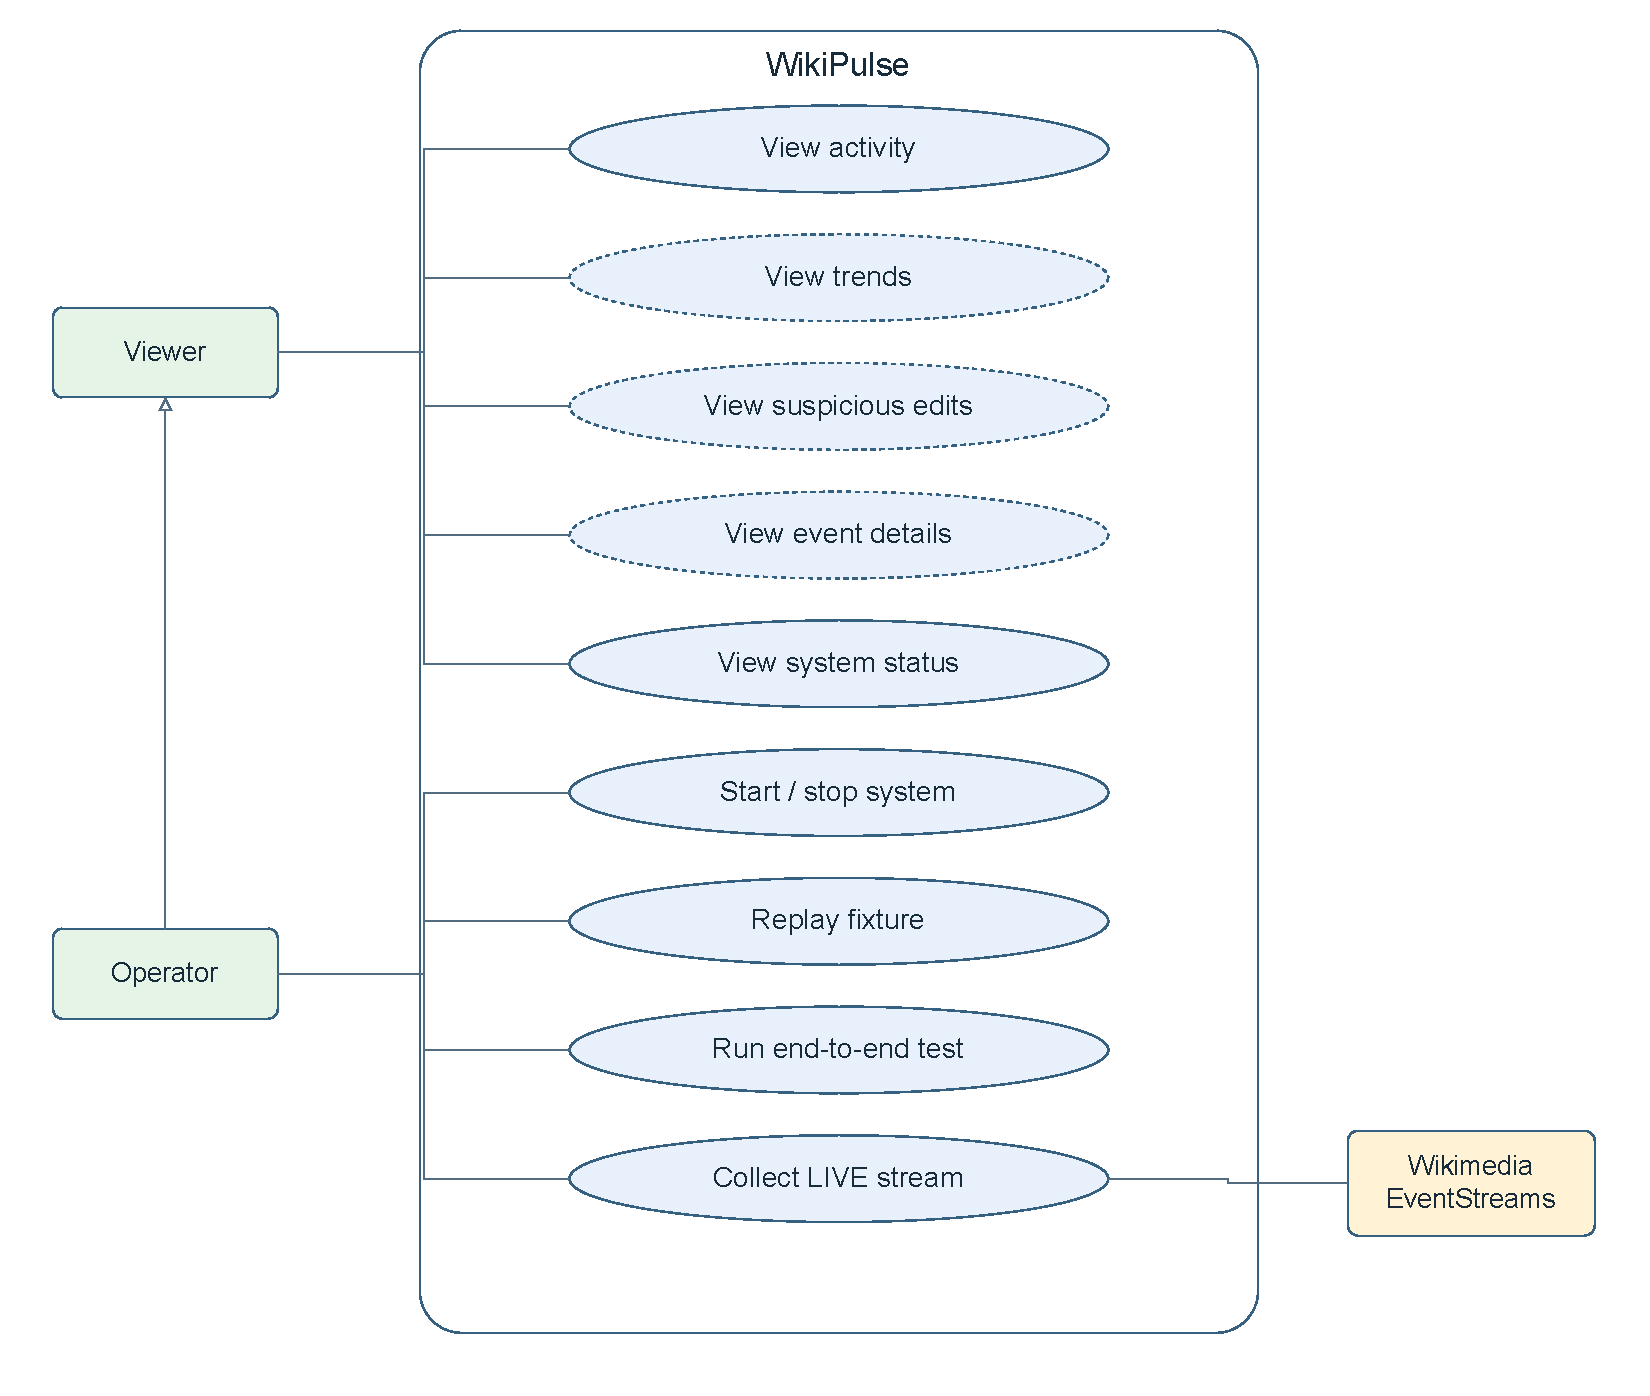
\includegraphics[width=\linewidth,height=0.68\textheight,keepaspectratio]{so-do/design-usecase.pdf}
\caption{Biểu đồ use case tổng quát. Đường nối là quan hệ giữa tác nhân và use case; mũi tên tam giác rỗng là quan hệ
khái quát hóa (người vận hành làm được mọi việc của người xem). Viền đứt nét đánh dấu phần giao diện chưa hoàn thiện;
collector LIVE đã được thử riêng, không suy ra LIVE end-to-end đã nghiệm thu.}\label{fig:usecase}
\end{figure}
\dukiensua{Mạnh đối chiếu trạng thái dashboard và use case trước khi chốt.}

\subsection{Đặc tả các use case chính}
\begin{table}[H]
\centering\small
\caption{Đặc tả use case \enquote{Xem hoạt động theo wiki}}\label{tab:uc-hoatdong}
\begin{tabularx}{\linewidth}{@{}>{\bfseries}p{3.2cm}X@{}}
\toprule
Tác nhân & Người xem \\
Tiền điều kiện & Hệ thống đang chạy \\
Luồng chính & 1. Người xem mở trang Overview, chọn wiki (mặc định enwiki).\newline
2. Dashboard gọi API lấy các cửa sổ 1 phút mới nhất của wiki đó.\newline
3. API đọc đúng partition của wiki trong Cassandra và trả kết quả, gắn nhãn \enquote{tạm tính}.\newline
4. Dashboard hiện năm chỉ số (sự kiện, chỉnh sửa, trang mới, sửa ẩn danh, sửa bởi bot) và biểu đồ theo thời gian;
tự làm mới sau 15 giây.\newline
5. Người xem có thể chọn một cửa sổ cụ thể để xem riêng. \\
Luồng thay thế & 3a. Chưa có dữ liệu: hiện thông báo trống, không hiện số giả.\newline
3b. Cassandra không phản hồi: API trả lỗi \enquote{phụ thuộc chưa sẵn sàng}; dashboard báo dịch vụ chưa sẵn sàng.\newline
1a. Wiki không nằm trong danh sách cho phép: API từ chối yêu cầu. \\
Hậu điều kiện & Không thay đổi dữ liệu \\
\bottomrule
\end{tabularx}
\end{table}

\begin{table}[H]
\centering\small
\caption{Đặc tả use case \enquote{Phát lại dữ liệu mẫu}}\label{tab:uc-replay}
\begin{tabularx}{\linewidth}{@{}>{\bfseries}p{3.2cm}X@{}}
\toprule
Tác nhân & Người vận hành \\
Tiền điều kiện & Kafka đã sẵn sàng và đã có topic \\
Luồng chính & 1. Người vận hành chạy lệnh phát lại.\newline
2. Hệ thống đọc từng dòng của file dữ liệu mẫu, giữ nguyên định danh và thời điểm của sự kiện, thêm thời điểm nhận.\newline
3. Hệ thống gửi từng sự kiện vào Kafka với khóa wiki và trang, chờ Kafka xác nhận.\newline
4. Spark xử lý sự kiện; nếu cấu hình và các dịch vụ phục vụ sẵn sàng, dashboard có thể hiển thị kết quả. \\
Luồng thay thế & 2a. Dòng không phải JSON hợp lệ: vẫn gửi nguyên văn để kiểm tra đường xử lý bản ghi hỏng.\newline
1a. Người vận hành chọn tốc độ phát nhanh hơn: chỉ đổi nhịp gửi, không đổi thời điểm sự kiện. \\
Hậu điều kiện & Kafka có thêm các sự kiện mẫu; Spark deduplicate theo event ID trong phạm vi watermark \\
\bottomrule
\end{tabularx}
\end{table}

\begin{table}[H]
\centering\small
\caption{Đặc tả use case \enquote{Xem trang xu hướng}}\label{tab:uc-xuhuong}
\begin{tabularx}{\linewidth}{@{}>{\bfseries}p{3.2cm}X@{}}
\toprule
Tác nhân & Người xem \\
Tiền điều kiện & Hệ thống đang chạy, Spark ghi kết quả xu hướng vào Cassandra \\
Luồng chính & 1. Người xem mở trang Trending, chọn wiki.\newline
2. Dashboard gọi API lấy top-N trang của cửa sổ 5 phút mới nhất.\newline
3. API tra bảng chỉ mục để biết cửa sổ mới nhất của wiki, đọc toàn bộ các trang trong cửa sổ đó, sắp theo điểm xu
hướng giảm dần (hòa thì theo số chỉnh sửa, rồi theo mã trang) và trả N dòng đầu kèm mốc đầu, cuối của cửa sổ.\newline
4. Dashboard hiện bảng trang xu hướng, gắn nhãn \enquote{tạm tính}. \\
Luồng thay thế & 2a. Người xem chọn một cửa sổ cụ thể: API đọc đúng cửa sổ đó.\newline
3a. Chưa có cửa sổ nào: trả danh sách rỗng, mốc cửa sổ để trống.\newline
3b. Cửa sổ có hơn 5.000 trang: API báo vượt dung lượng thay vì trả bảng xếp hạng bị cắt.\newline
3c. Cassandra không phản hồi: API báo \enquote{phụ thuộc chưa sẵn sàng}. \\
Hậu điều kiện & Không thay đổi dữ liệu \\
\bottomrule
\end{tabularx}
\end{table}

\begin{table}[H]
\centering\small
\caption{Đặc tả use case \enquote{Xem chỉnh sửa cần ưu tiên}}\label{tab:uc-uutien}
\begin{tabularx}{\linewidth}{@{}>{\bfseries}p{3.2cm}X@{}}
\toprule
Tác nhân & Người xem \\
Tiền điều kiện & Hệ thống đang chạy, Spark ghi các chỉnh sửa có điểm ưu tiên lớn hơn 0 vào Cassandra \\
Luồng chính & 1. Người xem mở trang Suspicious Edits, chọn wiki, số phút gần nhất (1--15) và điểm tối thiểu.\newline
2. Dashboard gọi API.\newline
3. API lấy danh sách các phút có chỉnh sửa đáng chú ý trong khoảng đã chọn từ bảng chỉ mục, đọc từng phút, lọc theo
điểm tối thiểu, sắp theo điểm rồi theo thời điểm giảm dần.\newline
4. Dashboard hiện danh sách kèm lý do (xóa nhiều nội dung, hoàn tác, sửa ẩn danh) và câu nhắc \enquote{điểm dùng để
ưu tiên xem xét, không kết luận phá hoại}. \\
Luồng thay thế & 3a. Không có chỉnh sửa nào: trả danh sách rỗng.\newline
3b. Tổng số dòng các phút cần đọc vượt 5.000: API báo vượt dung lượng.\newline
1a. Số phút hoặc điểm tối thiểu ngoài giới hạn: API từ chối, chỉ rõ tham số sai. \\
Hậu điều kiện & Không thay đổi dữ liệu; phản hồi không có trường user, IP, comment hoặc user hash; page title có thể chứa thông tin nhận dạng \\
\bottomrule
\end{tabularx}
\end{table}

\begin{table}[H]
\centering\small
\caption{Đặc tả use case \enquote{Xem chi tiết một sự kiện}}\label{tab:uc-chitiet}
\begin{tabularx}{\linewidth}{@{}>{\bfseries}p{3.2cm}X@{}}
\toprule
Tác nhân & Người xem \\
Tiền điều kiện & Người xem có định danh sự kiện, thường lấy từ danh sách chỉnh sửa cần ưu tiên \\
Luồng chính & 1. Người xem chọn một sự kiện.\newline
2. API đọc đúng một dòng theo định danh sự kiện.\newline
3. API trả thông tin trang, phiên bản cũ và mới, độ dài, chênh lệch byte, các cờ ẩn danh, bot, sửa nhỏ, điểm và lý
do ưu tiên. \\
Luồng thay thế & 2a. Không tìm thấy (sai định danh, hoặc sự kiện cũ hơn 7 ngày đã hết hạn lưu): API trả lỗi
\enquote{không tìm thấy sự kiện}.\newline
3a. Sự kiện không dính dấu hiệu nào: điểm 0, danh sách lý do rỗng. \\
Hậu điều kiện & Không thay đổi dữ liệu \\
\bottomrule
\end{tabularx}
\end{table}
\dukiensua{Bước hiển thị trên dashboard của ba use case trên làm ở W2-MANH-01; phần API đã chạy.}
\subsubsection{Đặc tả use case \enquote{Thu thập luồng thật (LIVE)}}
Collector kết nối Wikimedia EventStreams, nhận sự kiện qua SSE và gửi vào Kafka raw topic. Khi kết nối gián đoạn,
collector thử reconnect và gửi \code{Last-Event-ID} của sự kiện cuối đã được Kafka xác nhận theo thứ tự. Cursor chỉ
được giữ trong bộ nhớ process, vì vậy restart bắt đầu từ stream hiện tại. Việc nghiệm thu LIVE end-to-end của nhóm
vẫn còn chờ; kết quả collector riêng được trình bày trong chương kiểm thử.
\dukiensua{Đối chiếu contract và review cùng Thành, Linh trước khi nghiệm thu.}

\subsection{Yêu cầu chức năng}
\begin{table}[H]
\centering\small
\caption{Yêu cầu chức năng và trạng thái}\label{tab:ycchucnang}
\begin{tabularx}{\linewidth}{@{}lXl@{}}
\toprule
\textbf{Mã} & \textbf{Yêu cầu} & \textbf{Trạng thái} \\ \midrule
F1 & Phát lại dữ liệu mẫu vào Kafka, giữ nguyên định danh và thời điểm sự kiện & Đã làm \\
F2 & Nhận luồng thật từ Wikimedia, tự nối lại khi mất kết nối & Collector đã thử \\
F3 & Kiểm tra, tách riêng bản ghi hỏng, chuẩn hóa, loại trùng & Đã làm \\
F4 & Đếm hoạt động theo wiki, cửa sổ 1 phút; có số tạm tính và số đã chốt & Đã làm \\
F5 & Trang xu hướng: cửa sổ 5 phút trượt mỗi 1 phút, top-N theo wiki & API đã làm \\
F6 & Ưu tiên xem xét chỉnh sửa theo ba dấu hiệu: xóa nhiều nội dung, hoàn tác qua lại, sửa ẩn danh & API đã làm \\
F7 & Tra cứu chi tiết một sự kiện & API đã làm \\
F8 & Dashboard 4 trang: Overview, Trending, Suspicious Edits, System Status & Overview đã làm \\
F9 & Lưu ba tầng trên HDFS & Đã thử REPLAY \\
\bottomrule
\end{tabularx}
\end{table}
\dukiensua{Cập nhật trạng thái theo từng checkpoint.}

\subsection{Yêu cầu phi chức năng}
\begin{itemize}
  \item \textbf{Độ trễ:} số tạm tính hiện trên API trong 30--60 giây ở tải demo (mục tiêu, chưa đo). Số đã chốt chậm hơn
        theo watermark 10 phút.
  \item \textbf{Đúng khi chạy lại:} kiểm tra retry và restart theo từng fixture; không suy ra exactly-once giữa các sink.
  \item \textbf{Riêng tư:} Silver loại trường user/comment gốc và dùng salted hash cho user; page title và metadata
        vẫn có thể chứa thông tin nhận dạng. Pseudonymization không bảo đảm anonymity hoàn toàn.
  \item \textbf{Tái hiện:} lệnh và điều kiện được ghi trong plan; một số lượt cần artifact local hoặc môi trường riêng.
  \item \textbf{Tài nguyên:} chạy được trên máy 16 GB RAM, cấp cho Docker 6--8 GB.
\end{itemize}

\section{Kiến trúc tổng quan}
\begin{figure}[H]
\centering
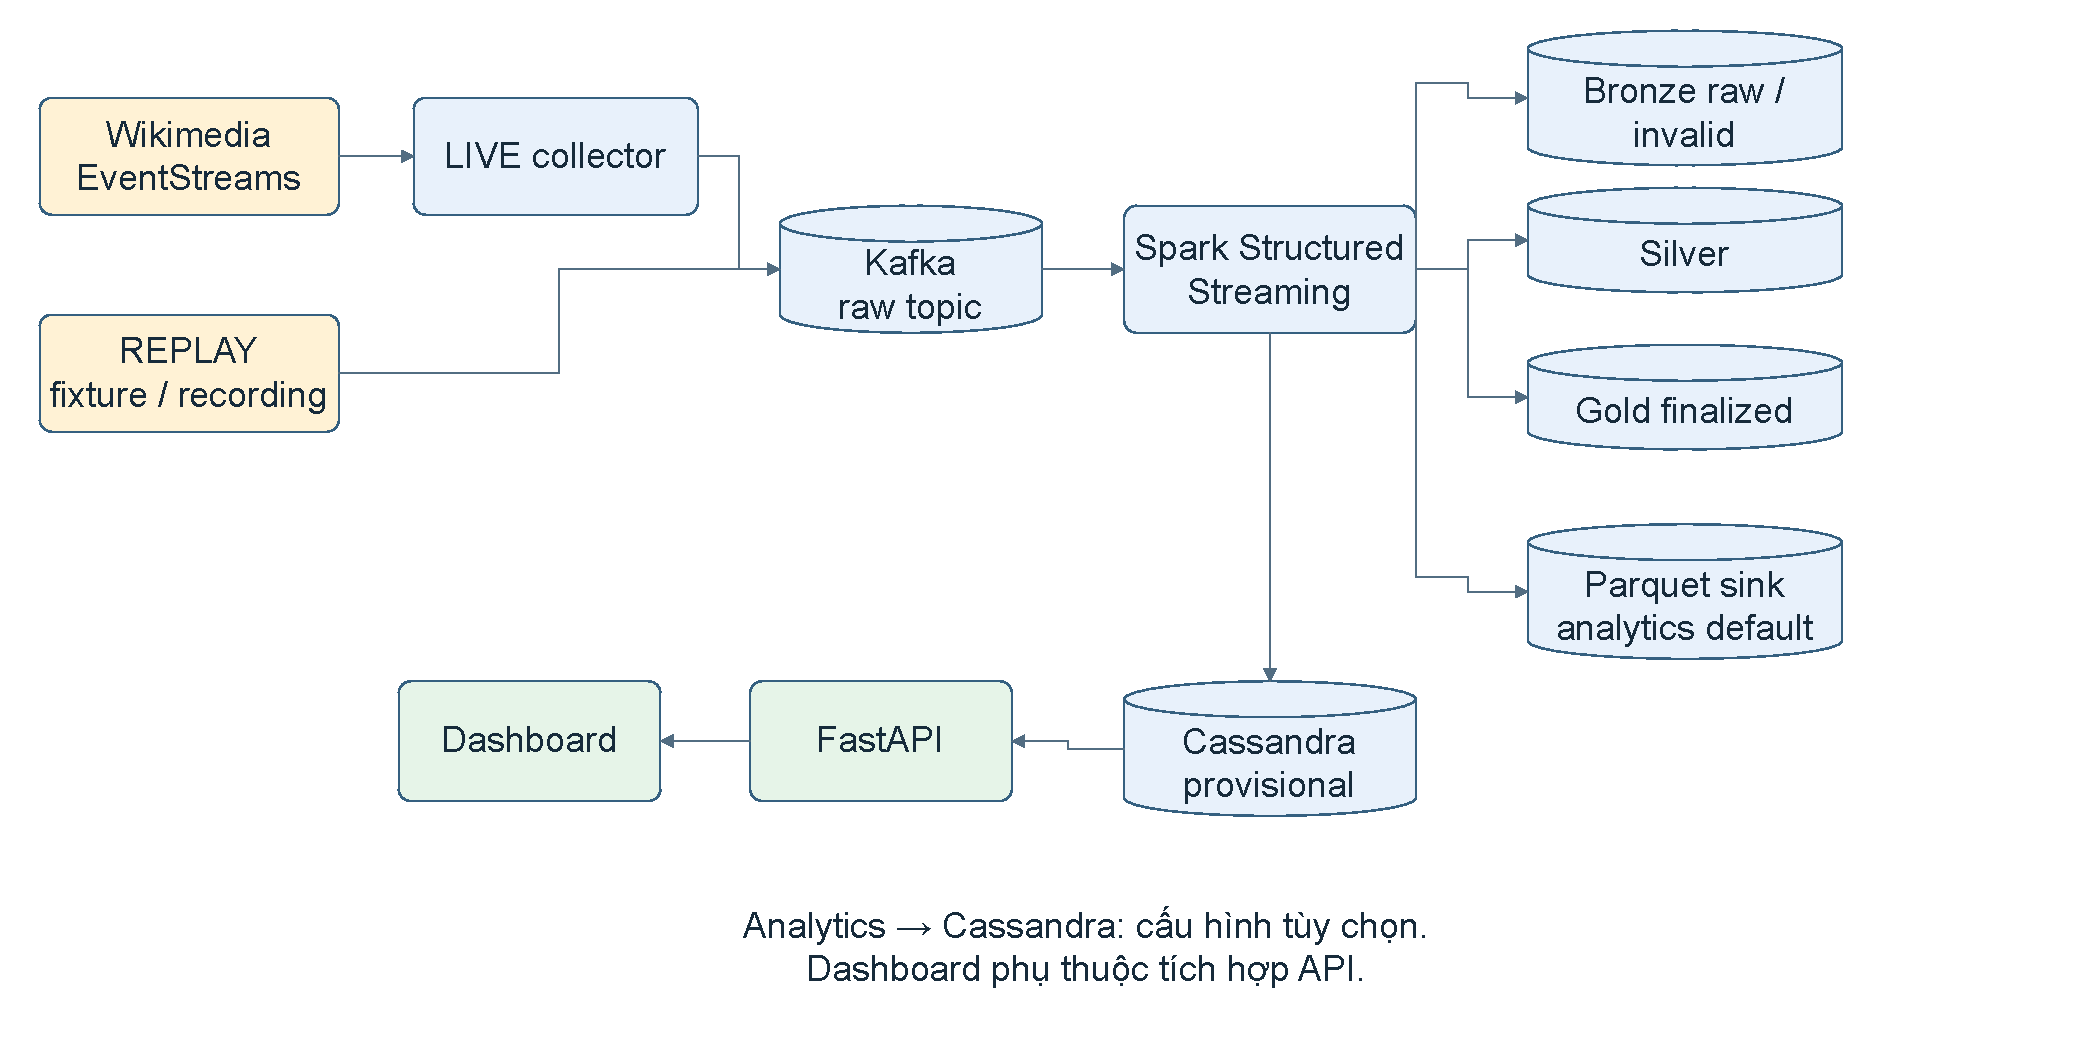
\includegraphics[width=\linewidth,height=0.68\textheight,keepaspectratio]{so-do/design-architecture.pdf}
\caption{Sơ đồ kiến trúc tổng quan. Collector LIVE đã được thử riêng với Kafka; sơ đồ không khẳng định toàn bộ luồng
LIVE tới dashboard đã được nghiệm thu. Màu xanh dương là xử lý, xanh lá là đầu ra, vàng là nguồn bên ngoài.}\label{fig:kientruc}
\end{figure}

Kafka tách phần nhận khỏi phần xử lý; Spark chuẩn hóa và tính các kết quả nghiệp vụ, API và dashboard đọc kết quả.
Dashboard gọi API thay vì đọc Cassandra trực tiếp. Theo cấu hình mặc định, analytics sink là Parquet; Cassandra cho
trends, suspicious edits và event detail phải được chọn trong cấu hình. API đã cài đặt không đồng nghĩa dashboard đã
kết nối đầy đủ hoặc dữ liệu có sẵn trong cấu hình mặc định.

\subsection{Các thành phần và người phụ trách}
\begin{table}[H]
\centering\small
\caption{Các thành phần (vị trí mã nguồn ở Phụ lục~\ref{app:ma})}\label{tab:module}
\begin{tabularx}{\linewidth}{@{}lXl@{}}
\toprule
\textbf{Thành phần} & \textbf{Nhiệm vụ} & \textbf{Phụ trách} \\ \midrule
Lõi dùng chung & Đọc và kiểm tra cấu hình, ghi log dạng JSON, lớp truy cập Cassandra & Trọng, Nhân \\
Thu thập & Phát lại dữ liệu mẫu, thu thập luồng thật & Thành \\
Xử lý & Tiến trình Spark: các truy vấn, phép biến đổi, giám sát truy vấn & Linh \\
Ghi kết quả & Đưa số đếm từ Spark vào Cassandra & Nhân \\
Phục vụ & Lược đồ Cassandra, API & Nhân \\
Giao diện & Dashboard và lớp gọi API & Mạnh \\
Tích hợp & Docker Compose, tạo topic, dữ liệu mẫu, kiểm thử end-to-end & Trọng \\
\bottomrule
\end{tabularx}
\end{table}

\subsection{Triển khai}
\begin{figure}[H]
\centering
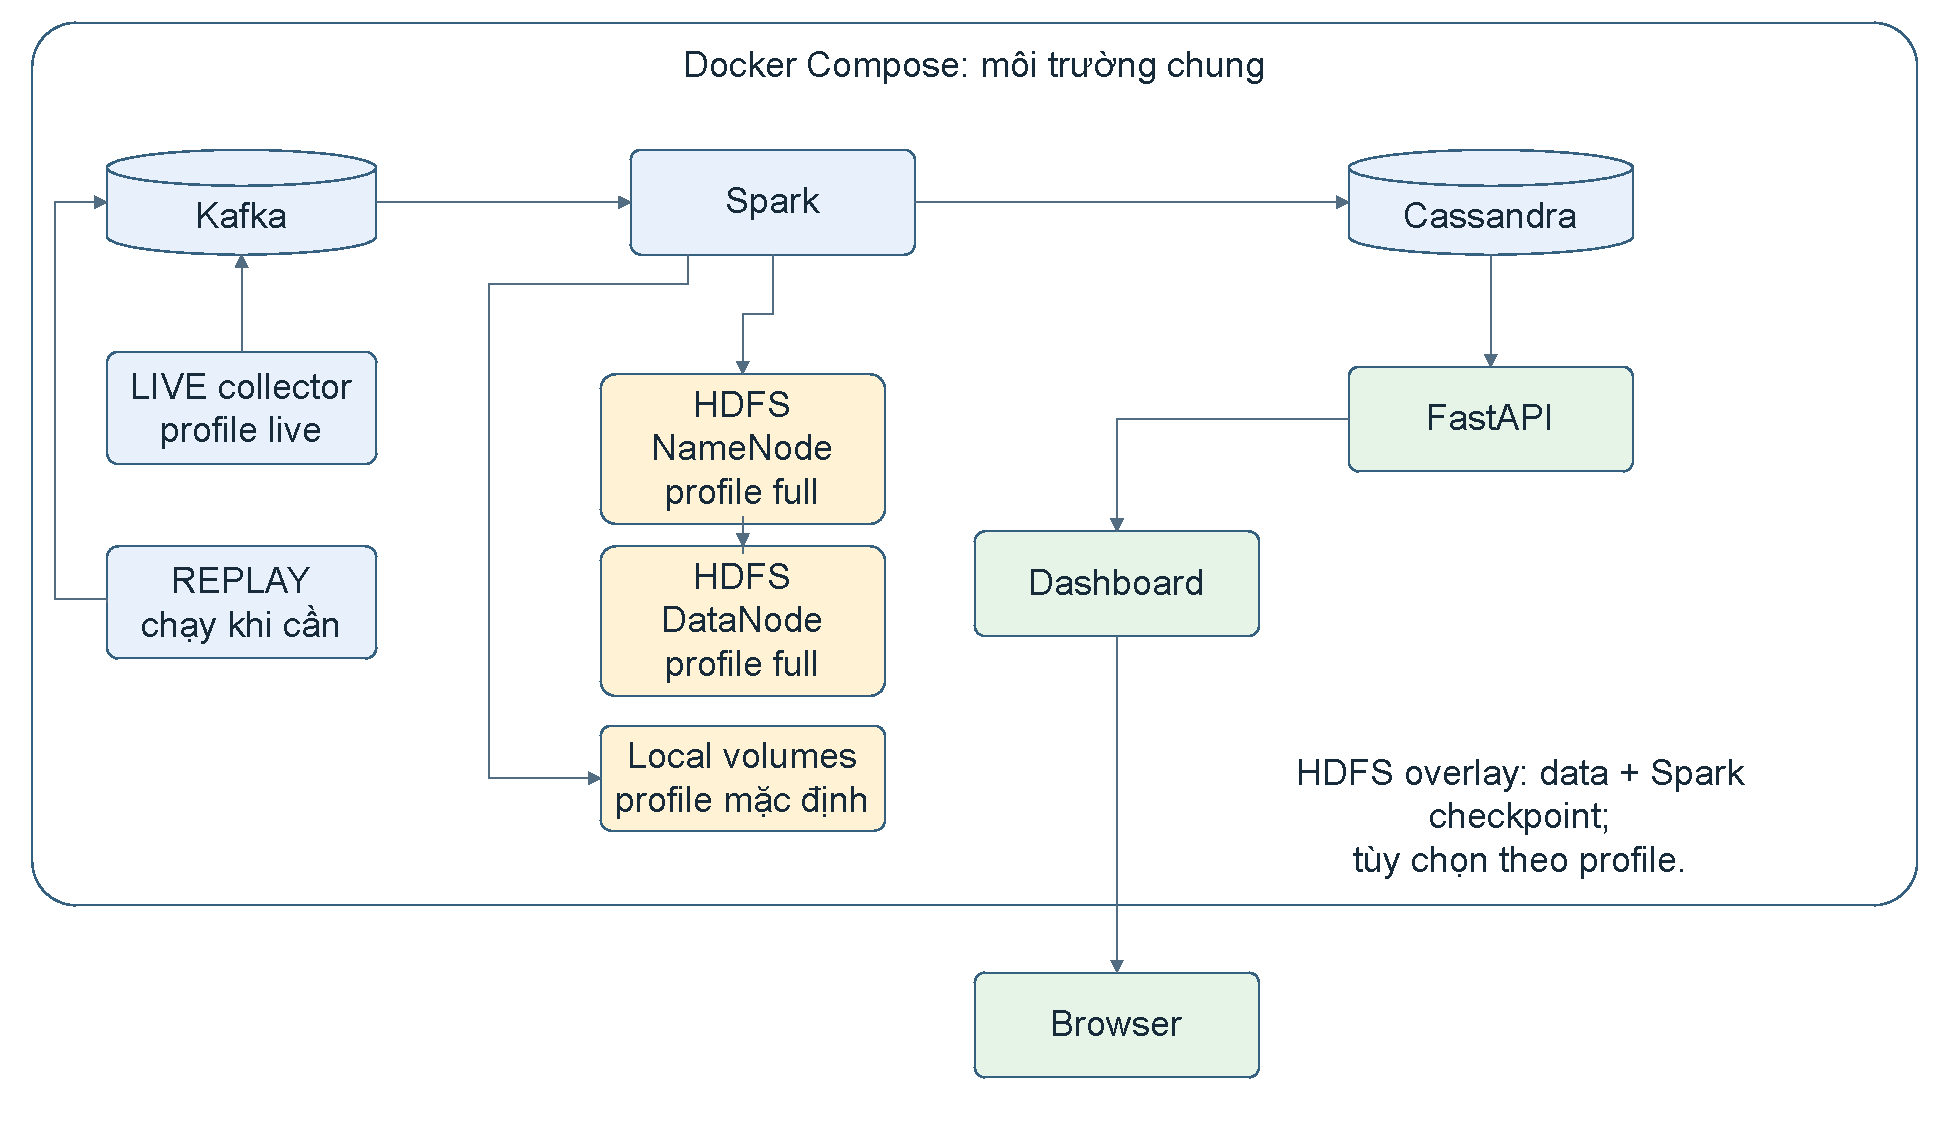
\includegraphics[width=\linewidth,height=0.68\textheight,keepaspectratio]{so-do/design-deployment.pdf}
\caption{Triển khai theo Docker Compose. Profile mặc định dùng local volume; profile full cùng HDFS overlay đưa dữ liệu và checkpoint vào HDFS.}\label{fig:trienkhai}
\end{figure}
Profile \code{full} bổ sung HDFS NameNode/DataNode; overlay HDFS chuyển dữ liệu Parquet và Spark checkpoint sang HDFS.
Profile mặc định dùng local volume. Kubernetes và monitoring mới có skeleton; không xem chúng là triển khai production.
\dukiensua{Trọng review hình triển khai và cấu hình profile.}

\section{Đường đi của một sự kiện}
Hình~\ref{fig:hoatdong} minh họa các bước kiểm tra trước khi một sự kiện được đếm. Bronze raw ghi các bản ghi Kafka mà query tương ứng đã đọc; các query là độc lập và không bảo đảm mọi sự kiện nguồn luôn được lưu.

\begin{figure}[H]
\centering
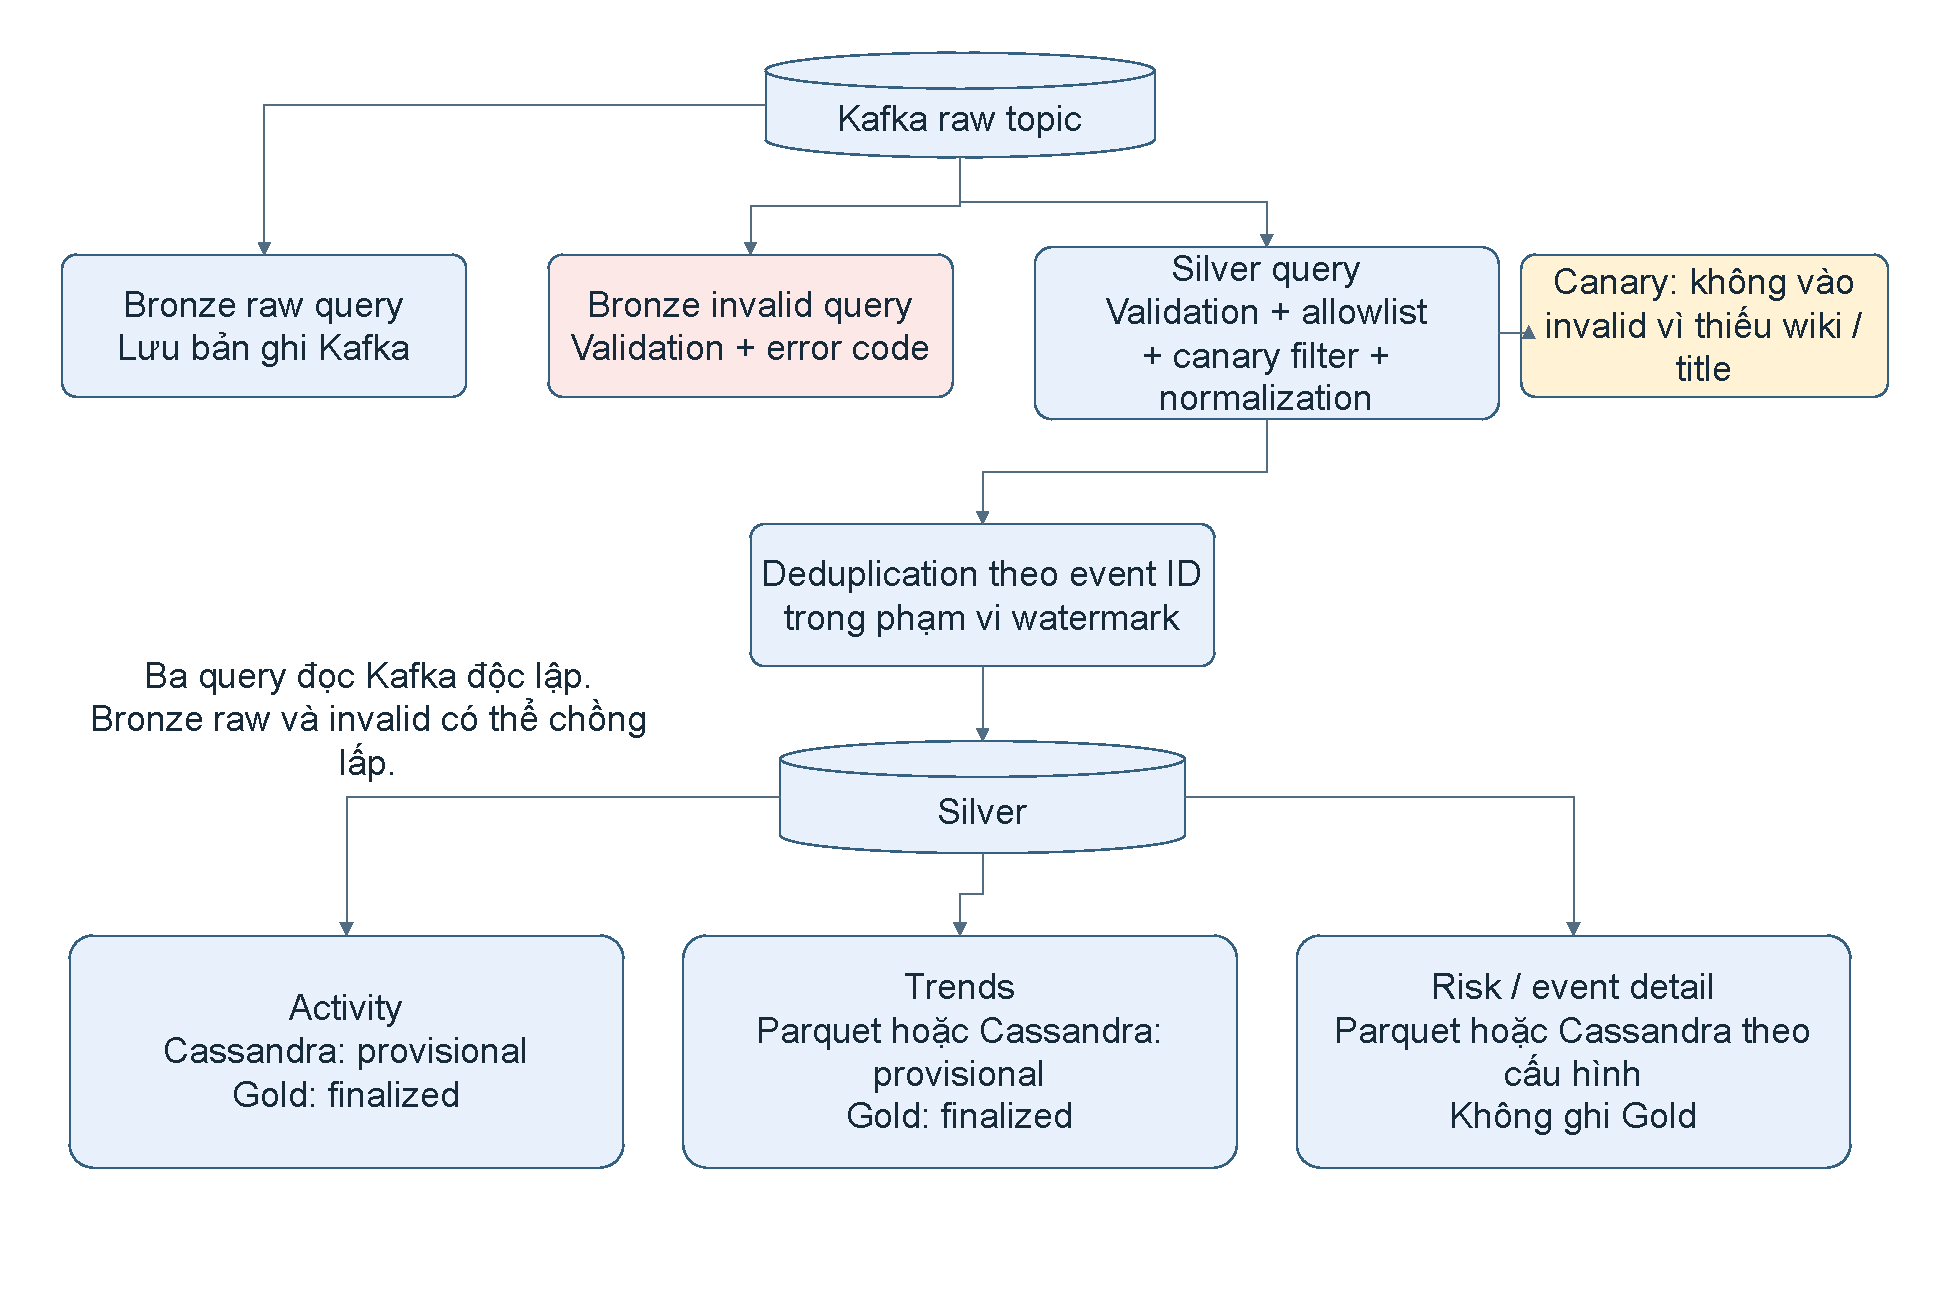
\includegraphics[width=\linewidth,height=0.68\textheight,keepaspectratio]{so-do/design-event-flow.pdf}
\caption{Các query đọc Kafka độc lập. Bronze raw và Bronze invalid có thể chồng lấp; Silver lọc canary và allowlist trước deduplication.}\label{fig:hoatdong}
\end{figure}

\section{Biểu đồ tuần tự: người xem mở trang Overview}\chualam
\dukiensua{Vẽ sau khi W1-MANH-01 xong, lúc luồng dashboard $\rightarrow$ API $\rightarrow$ Cassandra đã ổn định.}

\section{Cấu hình và tách lần chạy}
Mọi tham số (chế độ LIVE hay REPLAY, danh sách wiki, độ trễ watermark, địa chỉ các dịch vụ\ldots) được đọc từ biến môi
trường và kiểm tra ngay khi khởi động, trước khi mở kết nối tốn tài nguyên. Mỗi lần chạy có một \textbf{mã lần chạy};
dữ liệu và checkpoint của lần chạy nằm trong thư mục riêng mang mã đó, và mỗi truy vấn Spark có checkpoint riêng. Khi đổi
schema hay nguồn dữ liệu, nhóm tạo mã lần chạy và keyspace Cassandra mới chứ không xóa checkpoint rồi ghi tiếp vào kết quả
cũ. Kiểm thử end-to-end dùng mã lần chạy và vùng lưu trữ riêng nên không đụng dữ liệu đang dùng để phát triển.

\section{Thu thập dữ liệu}
\subsection{Kafka}
Hệ thống tạo ba topic cho raw, dead-letter queue (DLQ) và pipeline alerts; raw có ba partition, cấu hình demo có một
broker và replication factor 1. Topic DLQ đã tạo nhưng cách dùng Kafka DLQ sink còn chờ nhóm thống nhất; Bronze invalid
hiện lưu bản ghi lỗi. Với JSON object, envelope giữ trường nguồn và thêm \code{ingested\_at}, \code{collector\_version};
key là wiki và page ID, thiếu page ID thì dùng title. JSON sai hoặc không phải object được gửi nguyên văn không key.

\subsection{Phát lại dữ liệu mẫu}
Bộ phát lại đọc file dữ liệu mẫu và gửi từng dòng vào Kafka, giữ nguyên định danh và thời điểm sự kiện; tham số tốc độ
chỉ đổi nhịp gửi. Dữ liệu mẫu ngày 01/01/2026 có 11 dòng, được chọn để thử đủ các nhánh ở Hình~\ref{fig:hoatdong}: 5
chỉnh sửa enwiki, 1 trang mới viwiki, 1 bản trùng, 2 bản hỏng, 1 sự kiện canary, và 1 sự kiện lúc 00:12:10 để đẩy
watermark qua cửa sổ 00:00 (Hình~\ref{fig:watermark}).

Replay có thể dùng khoảng nghỉ cố định hoặc \code{original timing}. Với chế độ thứ hai, khoảng nghỉ dựa vào chênh lệch
event time hợp lệ và speed; event time và ID gốc không bị đổi. Dòng trống được bỏ qua, lỗi gửi làm lượt replay dừng.

\subsection{Thu thập luồng thật}
Collector đọc SSE từ Wikimedia, đóng gói sự kiện rồi gửi Kafka. Các ACK có thể về khác thứ tự; collector chỉ tiến
cursor sau chuỗi ACK thành công liên tiếp. Khi SSE ngắt, collector reconnect với backoff và dùng cursor hiện có làm
\code{Last-Event-ID}. Các event gần lỗi có thể được gửi lại; việc restart process không khôi phục cursor. Vì vậy không
cam kết exactly-once hoặc không mất sự kiện trong mọi tình huống.

\begin{figure}[H]
\centering
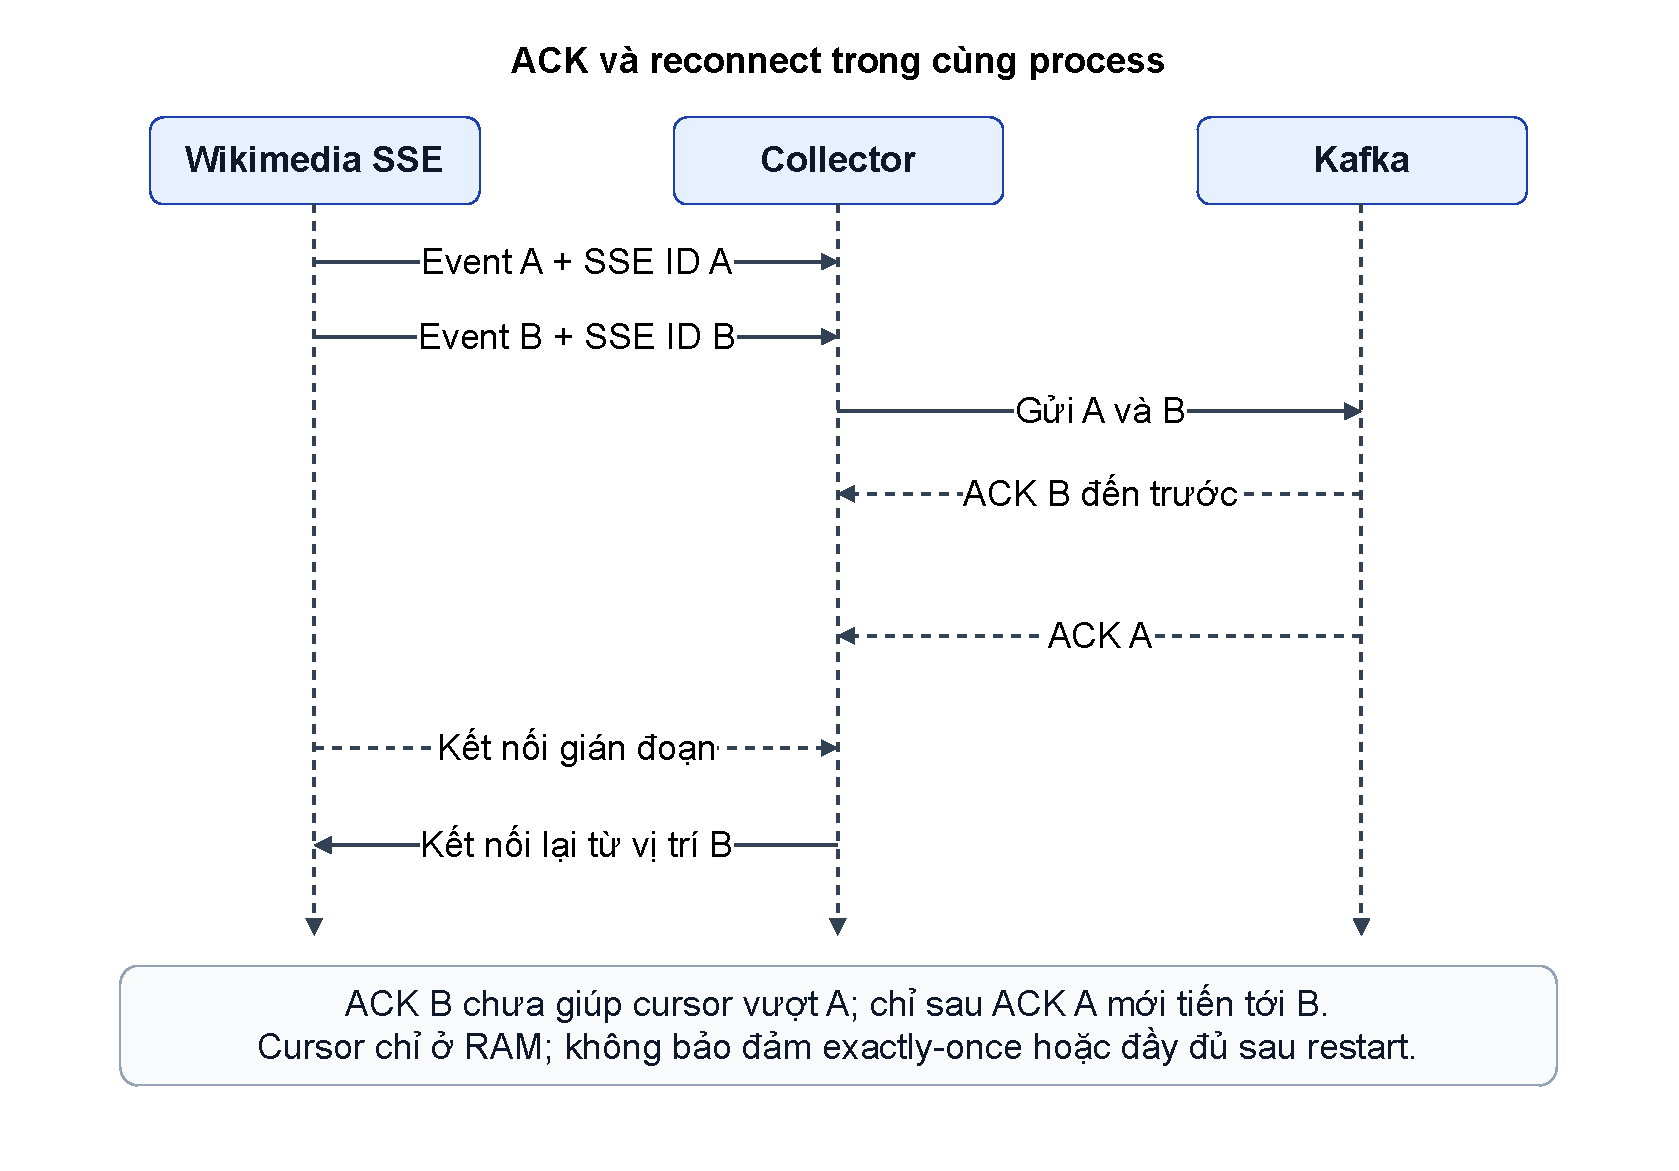
\includegraphics[width=\linewidth,height=0.55\textheight,keepaspectratio]{so-do/seq-ack.pdf}
\caption{ACK và reconnect: cursor chỉ tồn tại trong bộ nhớ process; hình không bảo đảm không mất hoặc không trùng sự kiện.}\label{fig:ack-reconnect}
\end{figure}

Recording là lựa chọn cục bộ: sau ACK liên tiếp, collector ghi bản sao chọn lọc, thay user bằng mã giả và loại comment
nguồn, chỉ giữ nhãn hoàn tác theo heuristic. Title và metadata vẫn có thể chứa danh tính; recording không phải anonymous
hoàn toàn và không được commit nguyên trạng. LIVE raw trong Kafka/Bronze vẫn có thể chứa user hoặc IP từ nguồn.
\dukiensua{Thành và Linh review mô tả collector/contract; nghiệm thu LIVE end-to-end còn chờ nhóm.}

\section{Xử lý luồng}\label{sec:spark}
\subsection{Các truy vấn}
Một tiến trình Spark chạy chín query độc lập trong cấu hình analytics, mỗi query có checkpoint riêng
(Bảng~\ref{tab:truyvan}). Silver được lưu trước khi các query đếm và analytics đọc lại. Cách này tách deduplication
khỏi aggregation và giúp khôi phục từng query theo checkpoint.

\begin{table}[H]
\centering\small
\caption{Các truy vấn streaming}\label{tab:truyvan}
\begin{tabularx}{\linewidth}{@{}lXl@{}}
\toprule
\textbf{Truy vấn} & \textbf{Việc làm} & \textbf{Ghi vào (chế độ)} \\ \midrule
Bronze thô & Đọc Kafka, giữ nguyên bản ghi và vị trí trong Kafka & Parquet (append) \\
Bronze hỏng & Đọc Kafka, lọc bản ghi hỏng, gắn mã lỗi & Parquet (append) \\
Silver & Đọc Kafka, lọc, chuẩn hóa, loại trùng & Parquet (append) \\
Hoạt động tạm tính & Đọc Silver, đếm theo wiki và phút & Cassandra (update) \\
Hoạt động đã chốt & Đọc Silver, đếm như trên & Parquet Gold (append) \\
Trends provisional & Đọc Silver, tính xu hướng theo window & Parquet hoặc Cassandra (update) \\
Suspicious edits & Đọc Silver, chọn edit có risk score lớn hơn 0 & Parquet hoặc Cassandra (append) \\
Event details & Đọc Silver, tạo chi tiết sự kiện & Parquet hoặc Cassandra (append) \\
Trends finalized & Đọc Silver, tính xu hướng đã chốt & Parquet Gold (append) \\
\bottomrule
\end{tabularx}
\end{table}

\subsection{Event ID và deduplication}
Định danh của sự kiện lấy từ nguồn. Nếu nguồn không có, hệ thống tự tạo bằng cách băm các trường không đổi của sự kiện
(wiki, trang, phiên bản, thời điểm, loại); không bao giờ dùng thời điểm nhận hay xử lý, vì như vậy cùng một sự kiện gửi
hai lần sẽ có hai định danh khác nhau. Mọi phép biến đổi dùng hàm có sẵn của Spark, không viết hàm Python riêng, để Spark
tối ưu được và không phải chuyển dữ liệu qua lại giữa Java và Python.

\subsection{Đếm hoạt động}
Với mỗi wiki và mỗi phút, hệ thống đếm: tổng sự kiện hợp lệ, số chỉnh sửa, số trang mới, và trong số chỉnh sửa thì bao
nhiêu là ẩn danh, bao nhiêu là của bot.

\subsection{Đặc trưng xu hướng}
Với từng wiki và trang, Spark tính trên window 5 phút trượt mỗi phút: số edit, số editor ước lượng bằng
\code{approx\_count\_distinct} trên user hash, và tổng độ lớn byte delta. Trend score kết hợp ba đặc trưng sau chuẩn hóa
và giới hạn theo cấu hình. Metadata của trang được chọn theo thứ tự ổn định của event time, event ID, title, namespace,
không theo thứ tự nhận. Kết quả provisional có thể thay đổi; Gold finalized được ghi khi watermark cho phép.

\subsection{Chấm điểm ưu tiên xem xét}
Risk score chỉ áp dụng cho event type edit. Cấu hình mặc định cộng 30 điểm khi xóa ít nhất 500 byte, 20 điểm khi comment
khớp heuristic revert tiếng Anh và 10 điểm cho anonymous edit không phải bot; tổng bị chặn theo mức cấu hình. Một edit
có thể khớp nhiều dấu hiệu. Điểm này hỗ trợ ưu tiên xem xét, không kết luận chỉnh sửa là phá hoại.
\dukiensua{Linh review mô tả scoring, watermark và ví dụ fixture trước khi chốt báo cáo.}

\section{Lưu trữ}
\subsection{Tầng Parquet}
Bronze và Silver chia thư mục theo ngày và giờ của sự kiện; Gold chia theo ngày, giờ và wiki. Danh sách đầy đủ các trường
của Silver nằm trong tài liệu contract của nhóm.
Parquet có thể lưu trên local volume hoặc HDFS theo cấu hình; các query dùng checkpoint riêng. Bài thử HDFS và phục hồi
trên fixture được trình bày ở chương kiểm thử, không mặc định đại diện cho tải production.

\subsection{Lược đồ Cassandra}\label{sec:cassandra}
Bảng hoạt động theo cửa sổ (Hình~\ref{fig:bangcass}) phục vụ đúng hai câu hỏi của API: \enquote{các phút mới nhất của
một wiki} và \enquote{một phút cụ thể của một wiki}. Cách chọn khóa đã giải thích ở Hình~\ref{fig:cassandra}.

\begin{figure}[H]
\centering
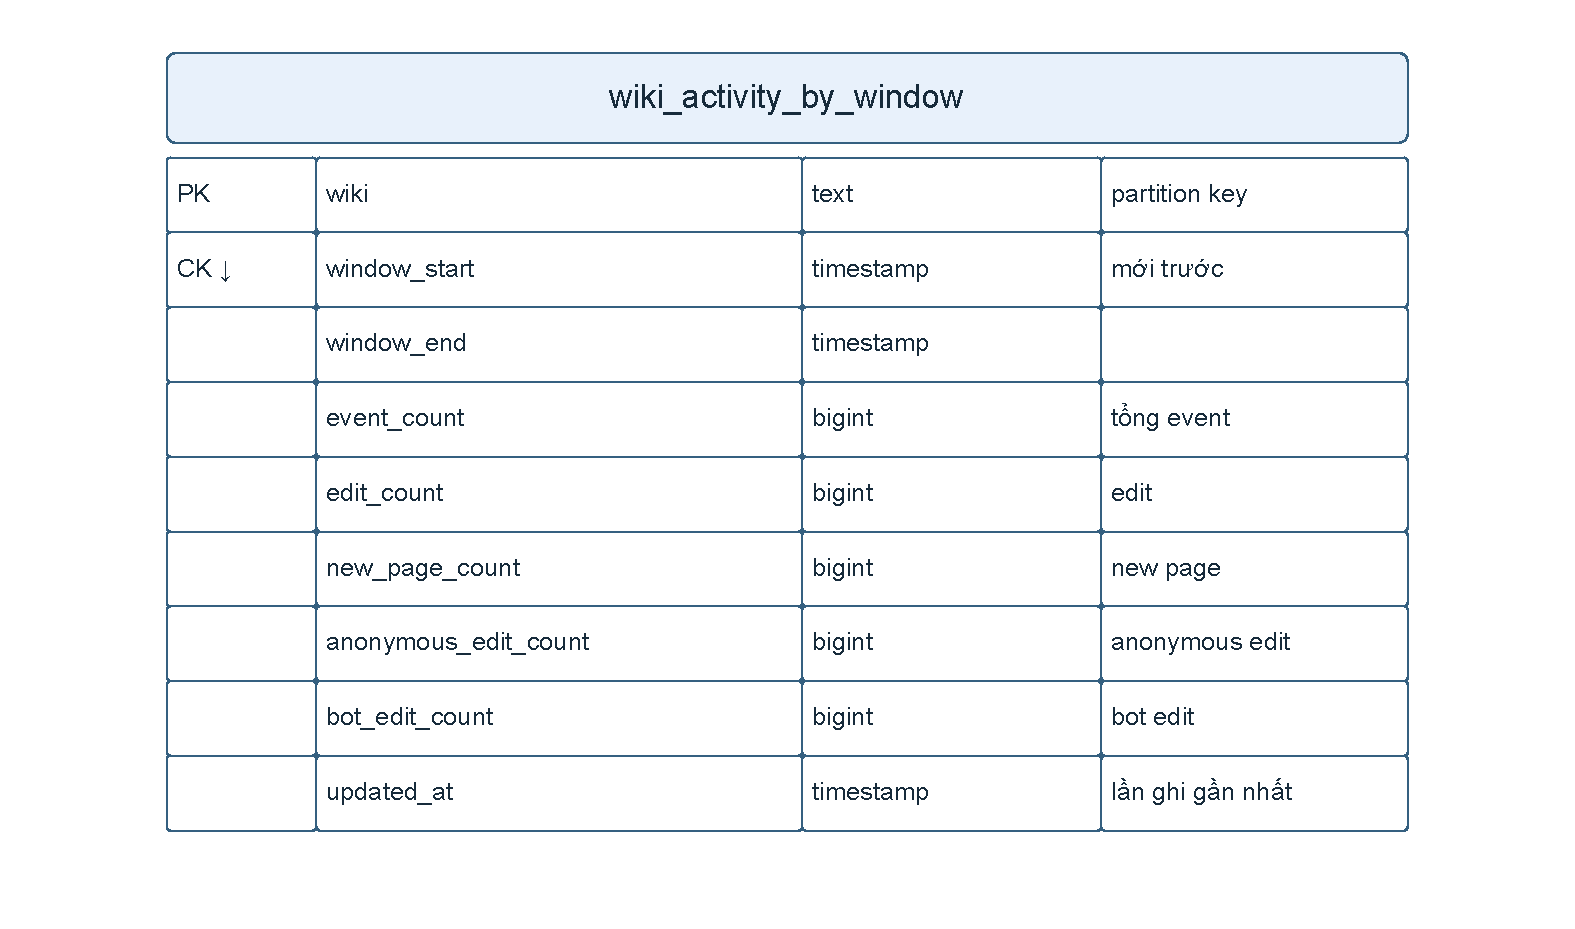
\includegraphics[width=\linewidth,height=0.68\textheight,keepaspectratio]{so-do/design-cassandra-activity.pdf}
\caption{Bảng hoạt động theo cửa sổ. PK: khóa partition; CK$\downarrow$: khóa sắp xếp, giảm dần.}\label{fig:bangcass}
\end{figure}

\begin{itemize}
  \item Spark ghi \textbf{tổng số} của cửa sổ, không ghi phần cộng thêm, nên ghi lại sau sự cố không làm đếm đôi.
  \item Mỗi wiki thêm 1.440 dòng mỗi ngày, khoảng 525 nghìn dòng mỗi năm: đủ cho demo. Trước khi chạy LIVE dài ngày cần
        đặt thời hạn tự xóa (TTL) hoặc chia partition theo ngày.
  \item Trước khi ghi, mỗi dòng được kiểm tra: tên wiki hợp lệ, cửa sổ kết thúc sau khi bắt đầu, số đếm nhất quán (chỉnh
        sửa cộng trang mới không vượt tổng; ẩn danh, bot không vượt số chỉnh sửa). Dòng sai làm batch thất bại;
        batch có thể được replay khi query/process được khởi động lại với checkpoint phù hợp.
\end{itemize}

Ba nghiệp vụ còn lại dùng năm bảng (Hình~\ref{fig:bangw2}). Mỗi query Cassandra cung cấp partition key; một API request
có thể đọc chỉ mục rồi truy vấn một hoặc nhiều partition, tùy nghiệp vụ. Các query không dùng \code{ALLOW FILTERING}.

\begin{figure}[H]
\centering
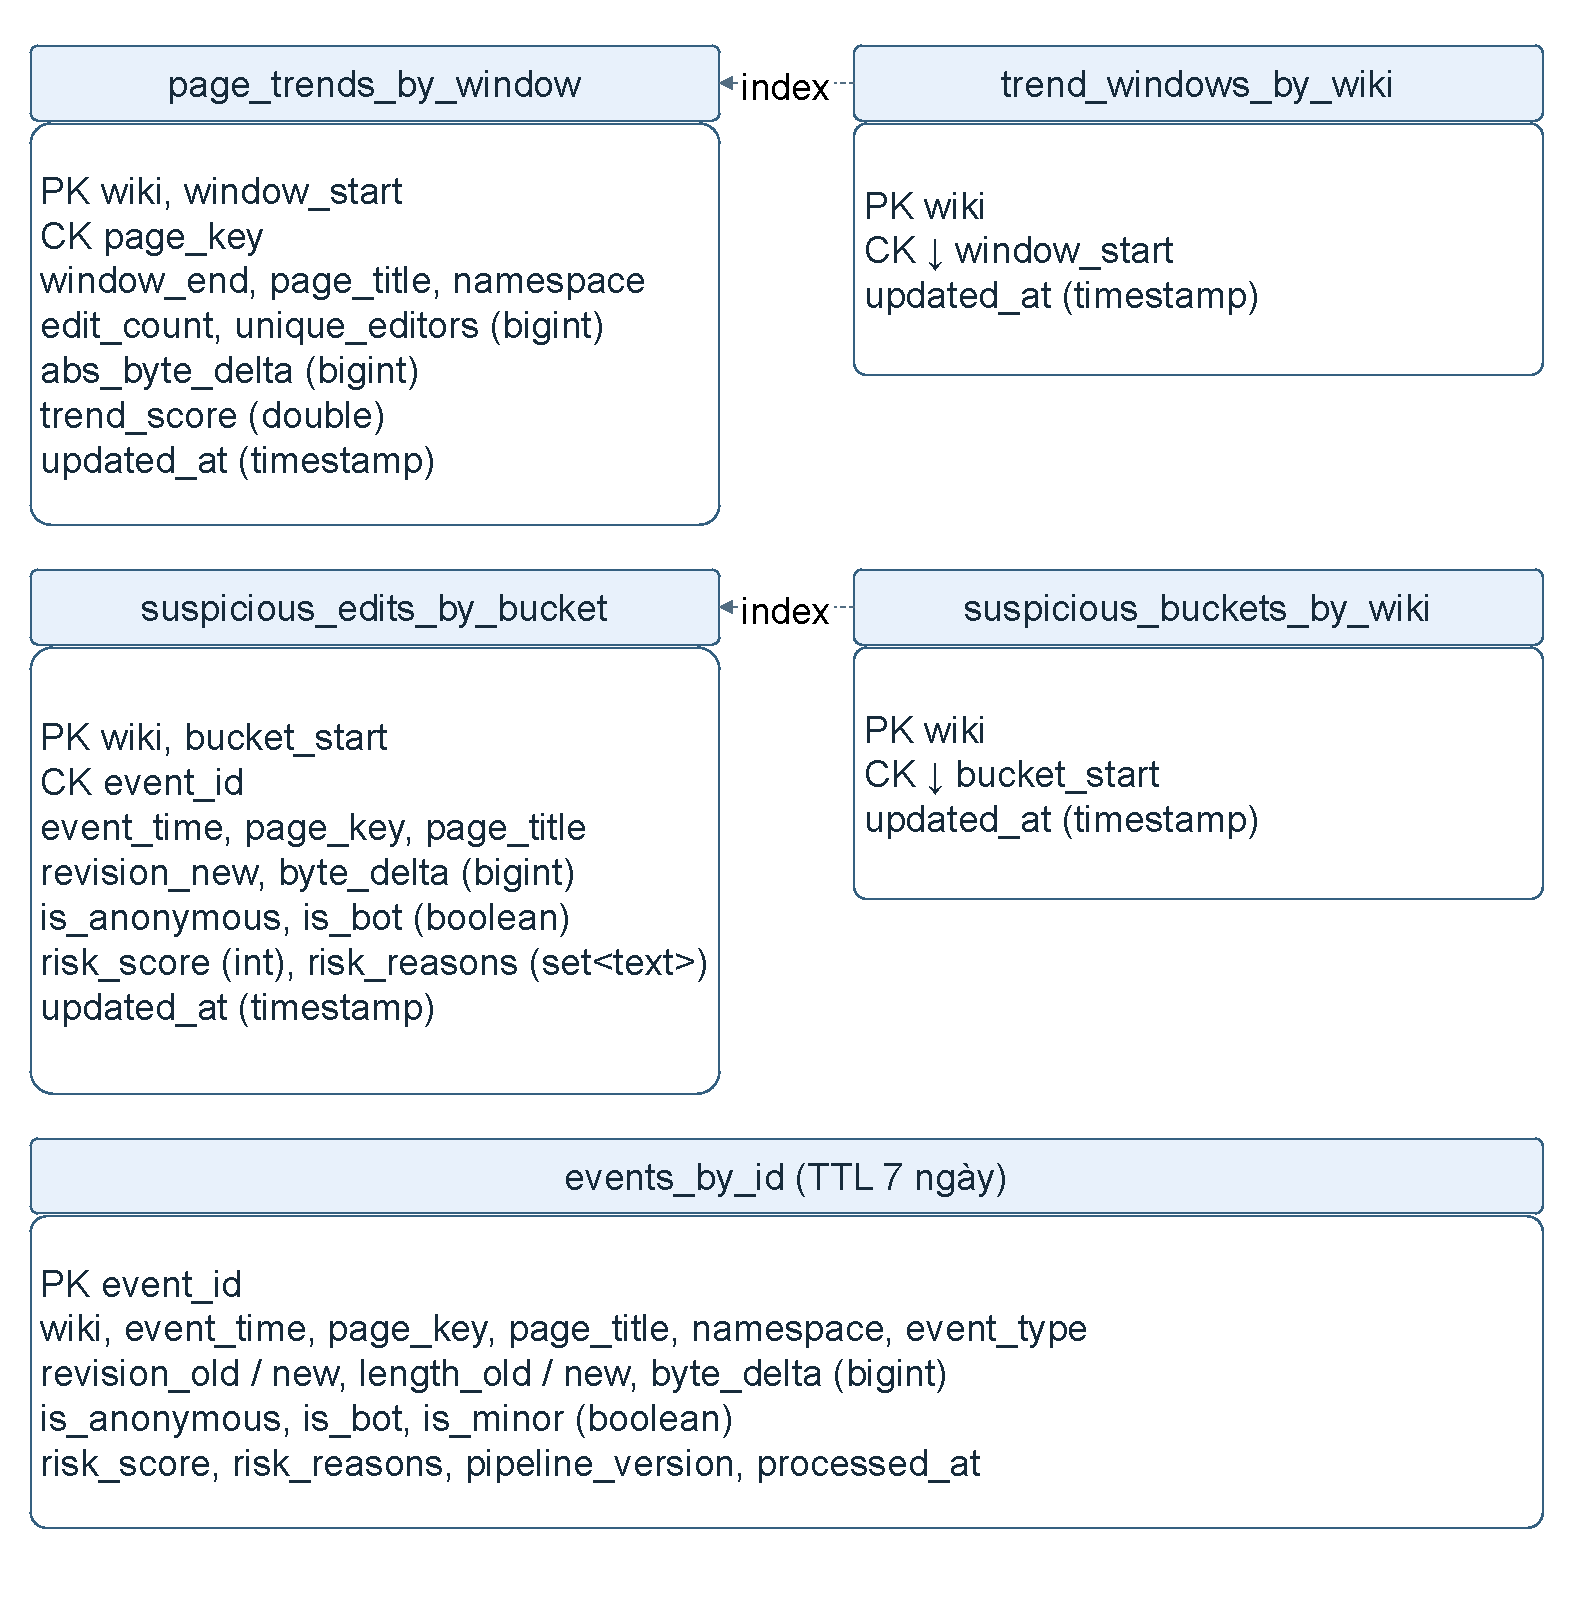
\includegraphics[width=\linewidth,height=0.68\textheight,keepaspectratio]{so-do/design-cassandra-analytics.pdf}
\caption{Năm bảng cho xu hướng, chỉnh sửa cần ưu tiên và chi tiết sự kiện. PK: khóa partition; CK: khóa sắp xếp
($\downarrow$ là giảm dần). Mũi tên nét đứt: bảng chỉ mục liệt kê các cửa sổ (hoặc phút) đã có dữ liệu ở bảng chính.}
\label{fig:bangw2}
\end{figure}

\begin{itemize}
  \item \textbf{Bảng chỉ mục thay cho quét bảng.} Cassandra không trả lời được \enquote{cửa sổ mới nhất của enwiki là cửa
        sổ nào} nếu chỉ có bảng chính, vì khóa partition gồm cả wiki lẫn mốc thời gian. Mỗi wiki vì vậy có thêm một
        partition liệt kê các cửa sổ (hoặc các phút) đã có dữ liệu, mới nhất trước.
  \item \textbf{Thứ tự ghi.} Trong mỗi batch, các dòng dữ liệu được ghi trước, chỉ mục ghi sau. Người đọc thấy một cửa sổ
        trong chỉ mục thì chắc chắn dữ liệu của cửa sổ đó đã có; batch hỏng giữa chừng và được chạy lại cũng chỉ ghi
        đè cùng các khóa.
  \item \textbf{Điểm không nằm trong khóa.} Điểm xu hướng và điểm ưu tiên thay đổi theo từng batch. Nếu đưa điểm vào khóa,
        mỗi lần điểm đổi sẽ sinh ra một dòng mới và dòng cũ vẫn còn. Vì vậy API đọc cả partition rồi tự sắp xếp.
  \item \textbf{Giới hạn 5.000 dòng.} Đọc cả partition chỉ an toàn khi partition nhỏ. API đọc tối đa 5.001 dòng; nếu
        thật sự có hơn 5.000 dòng thì báo vượt dung lượng chứ không trả bảng xếp hạng thiếu. Với chỉnh sửa cần ưu tiên,
        giới hạn tính trên tổng số dòng của mọi phút được đọc.
  \item \textbf{Hạn lưu chi tiết sự kiện.} Bảng chi tiết sự kiện tự xóa dòng sau 7 ngày. Lịch sử đầy đủ vẫn nằm ở Bronze
        và Silver; số đo làm căn cứ cho mốc 7 ngày ở Mục~\ref{sec:dungluong}.
  \item \textbf{Kiểm tra trước khi ghi.} Như bảng hoạt động, mỗi dòng phải đúng tập trường của contract (dòng có thêm định
        danh người dùng hay nội dung bình luận bị từ chối), cửa sổ xu hướng dài đúng 5 phút, phút của chỉnh sửa khớp
        thời điểm sự kiện, lý do ưu tiên thuộc ba mã đã định. Chỉ những trường Spark luôn điền mới bị kiểm tra bắt
        buộc, để một trường được phép trống không làm luồng thất bại lặp lại.
\end{itemize}

\subsection{Ghi kết quả từ Spark sang Cassandra}
Ở mỗi batch, tiến trình chính của Spark duyệt lần lượt từng dòng kết quả (không nạp cả batch vào bộ nhớ) và ghi vào
Cassandra. Nếu ghi lỗi, truy vấn dừng; khi query/process được khởi động lại với checkpoint phù hợp, batch có thể được replay. Parquet và Cassandra không có giao dịch
chung, nên hệ thống không cam kết \enquote{đúng một lần} trên cả hai nơi; tính đúng dựa vào việc ghi đè theo khóa ổn định.

\section{API}
\begin{table}[H]
\centering\small
\caption{Các endpoint}\label{tab:api}
\begin{tabularx}{\linewidth}{@{}lXl@{}}
\toprule
\textbf{Endpoint} & \textbf{Mô tả} & \textbf{Trạng thái} \\ \midrule
\code{/health} & Kiểm tra Cassandra thật sự trả lời được & Đã làm \\
\code{/api/v1/activity} & Hoạt động theo cửa sổ; chọn wiki, một cửa sổ cụ thể, số dòng tối đa 100 & Đã làm \\
\code{/api/v1/trends} & Top-N trang xu hướng của một cửa sổ 5 phút (mặc định cửa sổ mới nhất) & Đã làm \\
\code{/api/v1/suspicious-edits} & Chỉnh sửa cần ưu tiên trong 1--15 phút gần nhất, lọc theo điểm tối thiểu & Đã làm \\
\code{/api/v1/events/\{id\}} & Chi tiết một sự kiện & Đã làm \\
\bottomrule
\end{tabularx}
\end{table}

Các phản hồi dữ liệu kèm thời điểm tạo, nguồn và chế độ chạy; activity, trends và suspicious edits có nhãn \code{provisional}, còn event detail không có trường này. Mọi thời điểm theo UTC. Danh sách
không có dữ liệu được trả rỗng; event ID không tìm thấy trả 404. Tham số sai (wiki ngoài danh sách, cửa sổ thiếu múi giờ, số dòng ngoài
1--100) bị từ chối. Cassandra không trả lời thì API báo \enquote{phụ thuộc chưa sẵn sàng}; API vẫn khởi động được khi
Cassandra chưa lên và tự hồi phục khi Cassandra sẵn sàng. Danh sách chỉnh sửa cần ưu tiên luôn kèm câu nhắc điểm chỉ
để ưu tiên xem xét. API không trả các trường user, IP, comment hoặc user hash; page title vẫn có thể chứa thông tin nhận dạng.

Mọi lỗi có cùng một dạng: một mã lỗi cố định để chương trình đọc, một câu mô tả cho người đọc, và thông tin thêm tùy
loại (Bảng~\ref{tab:loi}). Lỗi tham số do thư viện web tự phát hiện (ví dụ số dòng bằng 0) cũng được đổi về dạng này,
để dashboard chỉ cần một cách đọc lỗi.

\begin{table}[H]
\centering\small
\caption{Các loại lỗi của API}\label{tab:loi}
\begin{tabularx}{\linewidth}{@{}llX@{}}
\toprule
\textbf{HTTP} & \textbf{Mã} & \textbf{Khi nào; thông tin thêm} \\ \midrule
422 & \code{INVALID\_QUERY} & Tham số sai; kèm danh sách tham số sai và lý do \\
404 & \code{EVENT\_NOT\_FOUND} & Không có sự kiện với định danh đã cho \\
503 & \code{DEPENDENCY\_UNAVAILABLE} & Cassandra không trả lời; kèm tên dịch vụ lỗi \\
503 & \code{CAPACITY\_EXCEEDED} & Phải đọc hơn 5.000 dòng để trả lời \\
\bottomrule
\end{tabularx}
\end{table}

\section{Dashboard}
Bốn trang: Overview (đọc dữ liệu activity theo wiki và cửa sổ 1 phút, tự làm mới sau 15 giây), Trending (Top-N trang tăng hoạt động trong cửa sổ 5 phút kèm liên kết Wikipedia), Suspicious Edits (danh sách chỉnh sửa ưu tiên xem xét với bộ lọc bot/điểm rủi ro và xem chi tiết sự kiện), và System Status (readiness của API và Cassandra). Giao diện không hiển thị các trường IP, username thô hay \code{user\_hash}; page title vẫn có thể chứa thông tin nhận dạng.
\dukiensua{Mạnh bổ sung ảnh chụp các trang mới (W2-MANH-01) và chuẩn hóa tên file ảnh không dấu/không khoảng trắng.}

% ============================================================================
% CHƯƠNG 5: KIỂM THỬ VÀ ĐÁNH GIÁ
% ============================================================================
